\documentclass[a4paper,12pt]{article}

\usepackage[english]{babel}
\usepackage{graphicx}
\usepackage{amsmath}

\title{Some simple algorithms for detecting anomalous bright pixels}
\author{Alessandro Gentilini}


\begin{document}
\maketitle

\begin{abstract}
I describe some simple algorithms I am using for detecting anomalous bright pixels in images taken by a laptop webcam.
The webcam lens is covered with black tape and so the visible light is not collected by the sensor; the grey levels different from zero in the image are usually due to the so called \emph{dark current}; sometimes there are bright pixels (and I classify the image as an \emph{event}) and an hypothesis is that the bright pixels are the result of the interaction of cosmic ray muons with the semiconductor sensor of the webcam.
\end{abstract} 

\section{Algorithms}
I am experimenting various algorithms in order to classify an image as an \emph{event}.

I have a sequence of images, let $I_i$ be the $i$-th image in the sequence. The image has $R$ rows and $C$ columns. Let $I_i(r,c)$ be the grey value of the pixel at $row=r$ and $column=c$ in the image $I_i$.
The program computes $M_i$ as 
$$M_i=\max_{\substack{
   0\leq r\leq R-1 \\
   0\leq c\leq C-1
  }}
 I_i(r,c)$$

So $M_i$ is the maximum grey level in the image $I_i$.

The simplest algorithm uses a fixed threshold $t$ and the image $I_i$ is classified as an event if 
\begin{equation}
M_i>t
\end{equation}

A different algorithm considers the average grey level $avg_i$ of the image $I_i$ and the standard deviation $sd_i$ of the grey levels of the image $I_i$, the image $I_i$ is then classified as an event if 
\begin{equation}
M_i>avg_i+n\cdot sd_i
\end{equation}

 In a third algorithm, the program keeps running statistics for $M_i$, in particular $\overline{M}_i$ is the mean of the maximum grey levels and it is computed as
 $$\overline{M}_i=\frac{1}{i}\sum_{k=1}^i M_k$$

 and ${\sigma_{M}}_{i}$ is the standard deviation of the maximum grey level and it is computed as

 $${\sigma_{M}}_{i}=\sqrt{\frac{1}{i(i-1)}\left(i\sum_{k=1}^i {M_k}^2-\left(\sum_{k=1}^i M_k\right)^2\right)}$$


The image $I_i$ is then considered an event if 
\begin{equation}
M_i>\overline{M}_i+n\cdot{\sigma_{M}}_{i}\label{eq:3}
\end{equation}

\begin{figure}[h!]
  \centering
  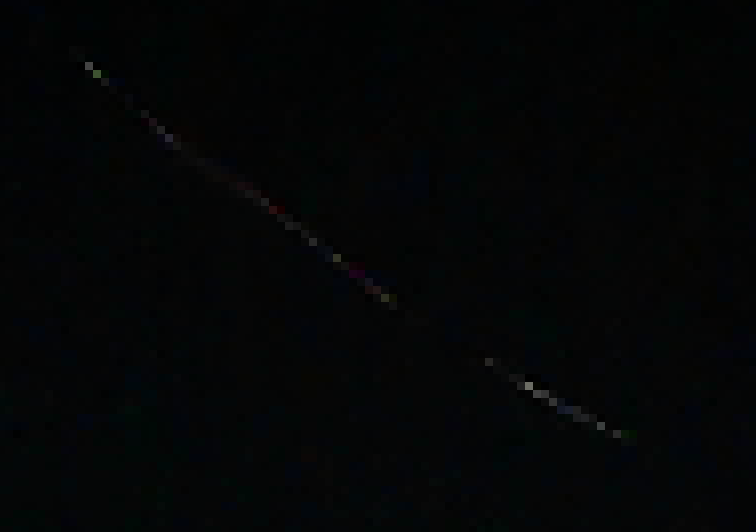
\includegraphics[scale=0.5]{bella.png}
  \caption{A crop from an image classified as an event using formula \ref{eq:3} with $n=10$.}
\end{figure}

\section{Data}
Figures \ref{fig:1} to \ref{fig:2} shows data collected in various days.
The time between two images acquisition has a mean value of 0.13s and a standard deviation of 7ms.
The exposure time is unknown.
The images were collected with a laptop webcam, the location is in Nothern Italy, the time is local.

\begin{figure}[h!]
  \centering
  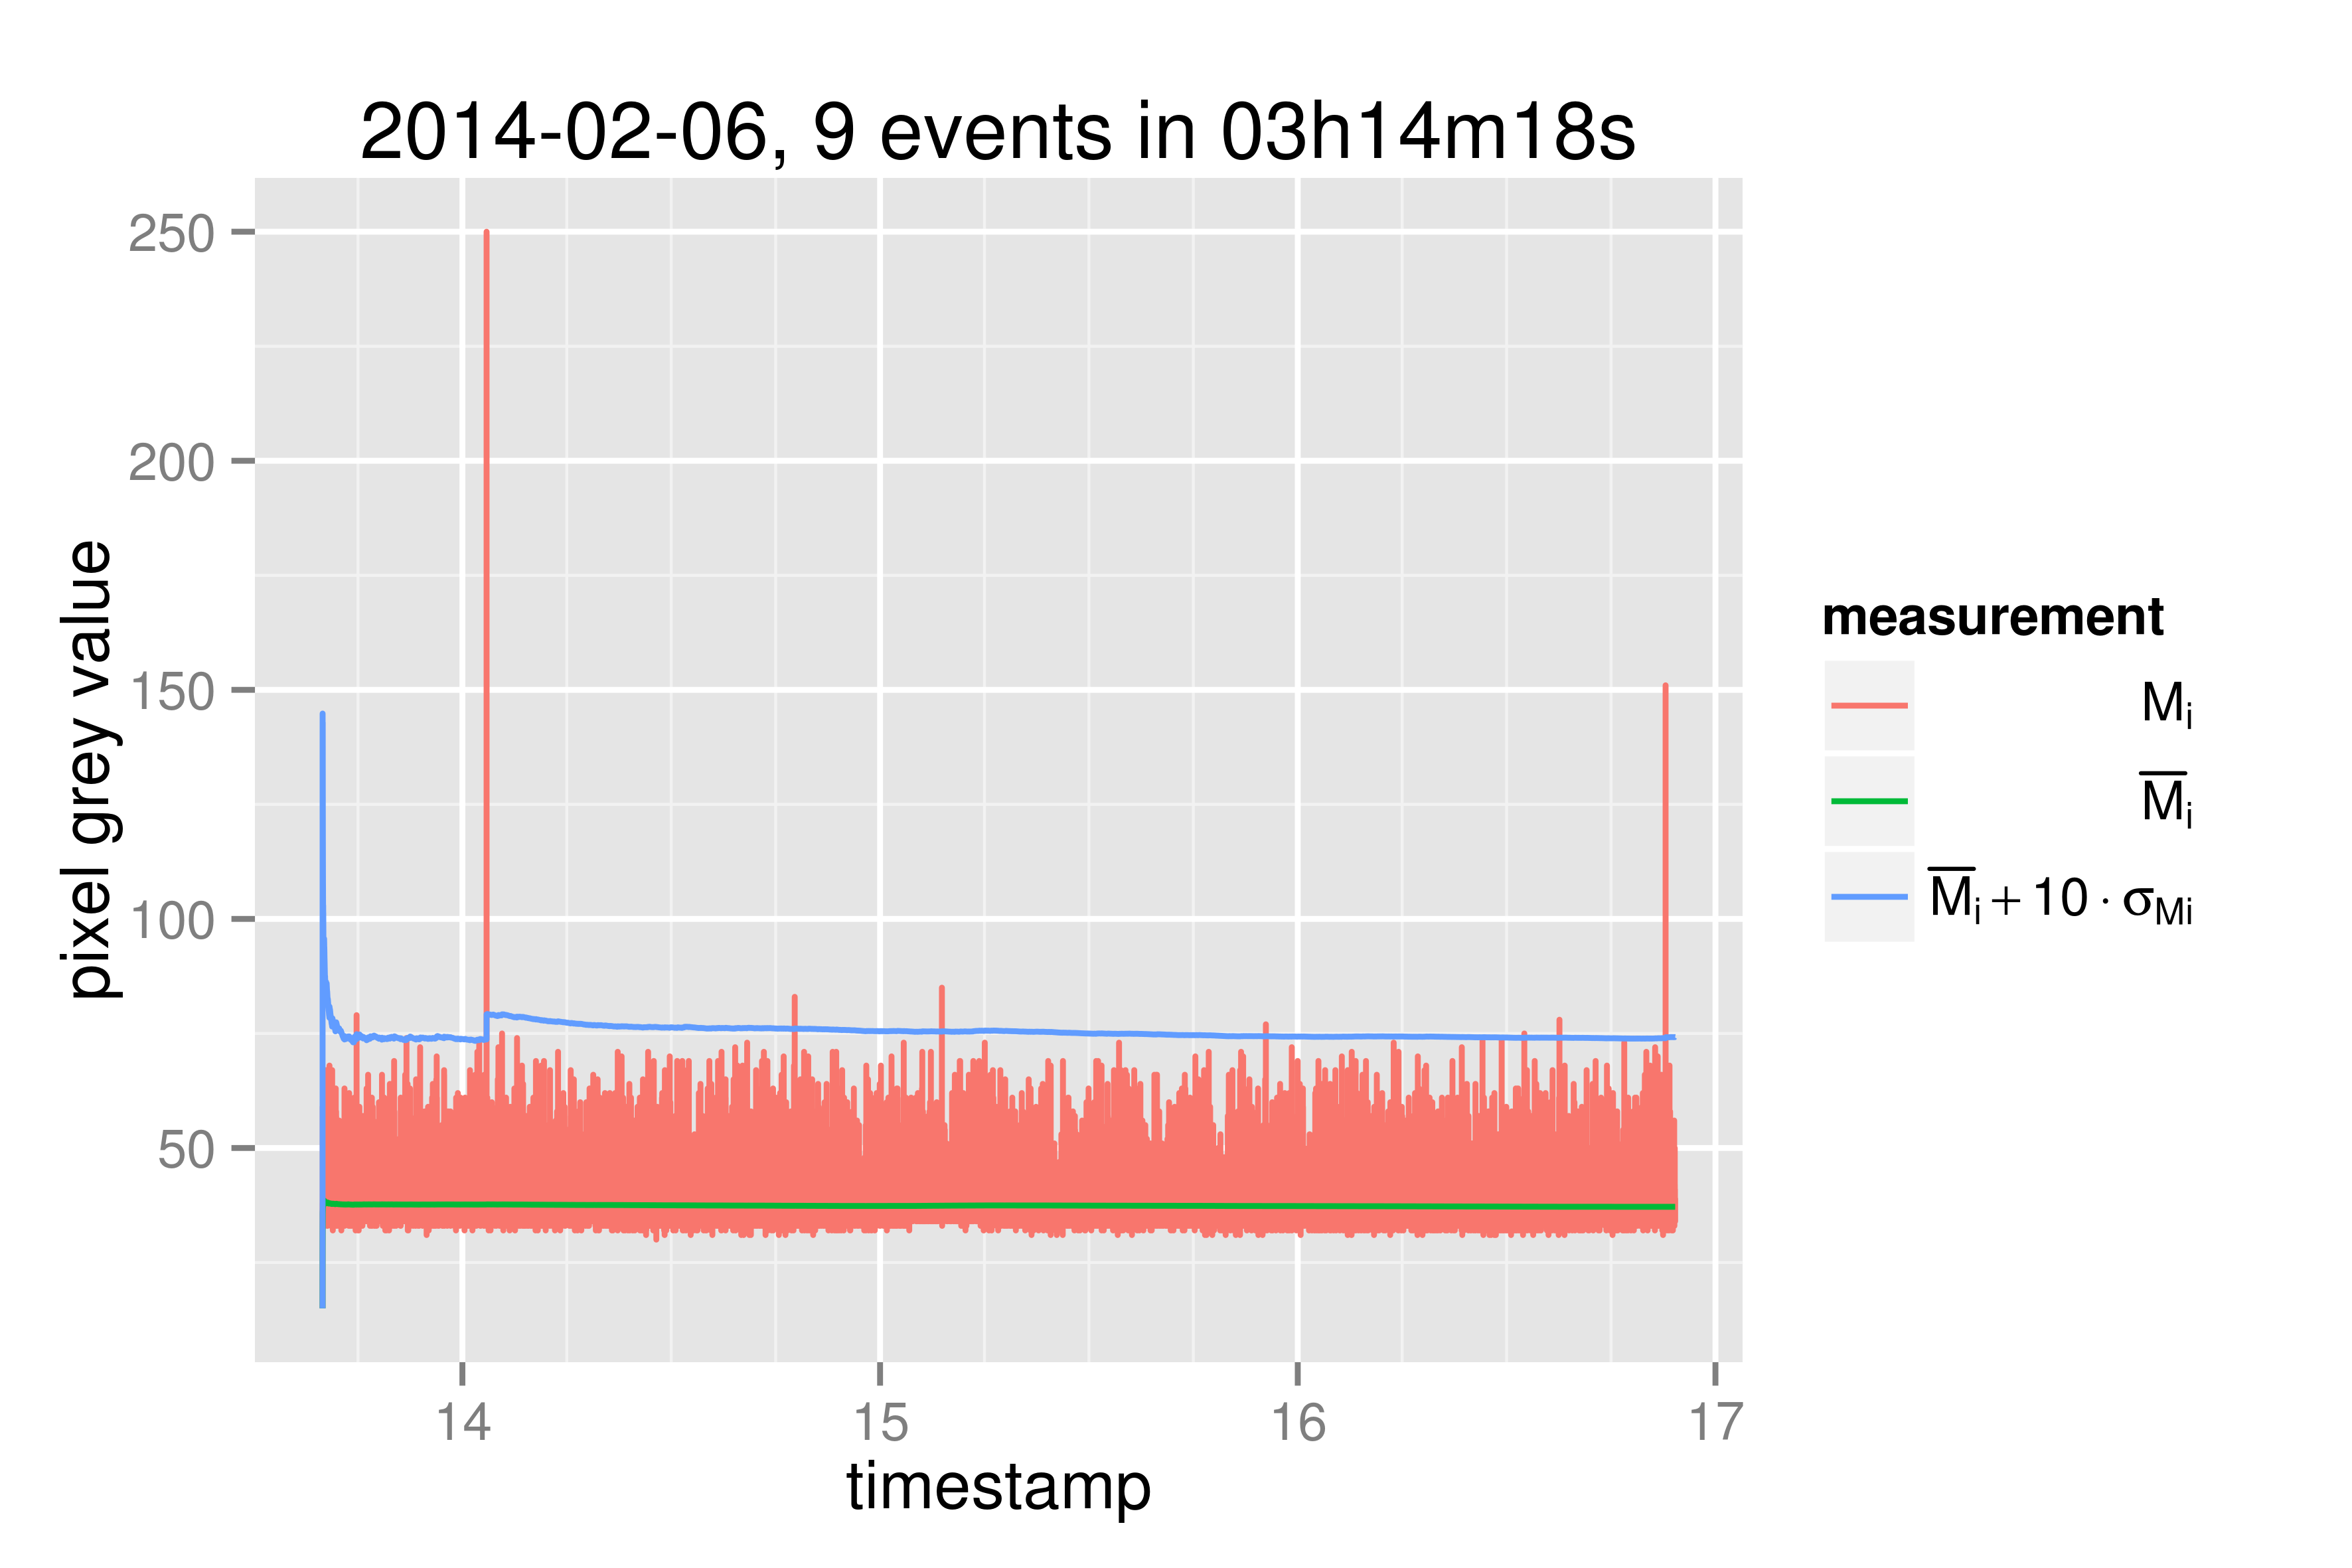
\includegraphics{20140206.png}
  \caption{Data collected using formula \ref{eq:3} with $n=10$.}\label{fig:1}
\end{figure}

\begin{figure}[h!]
  \centering
  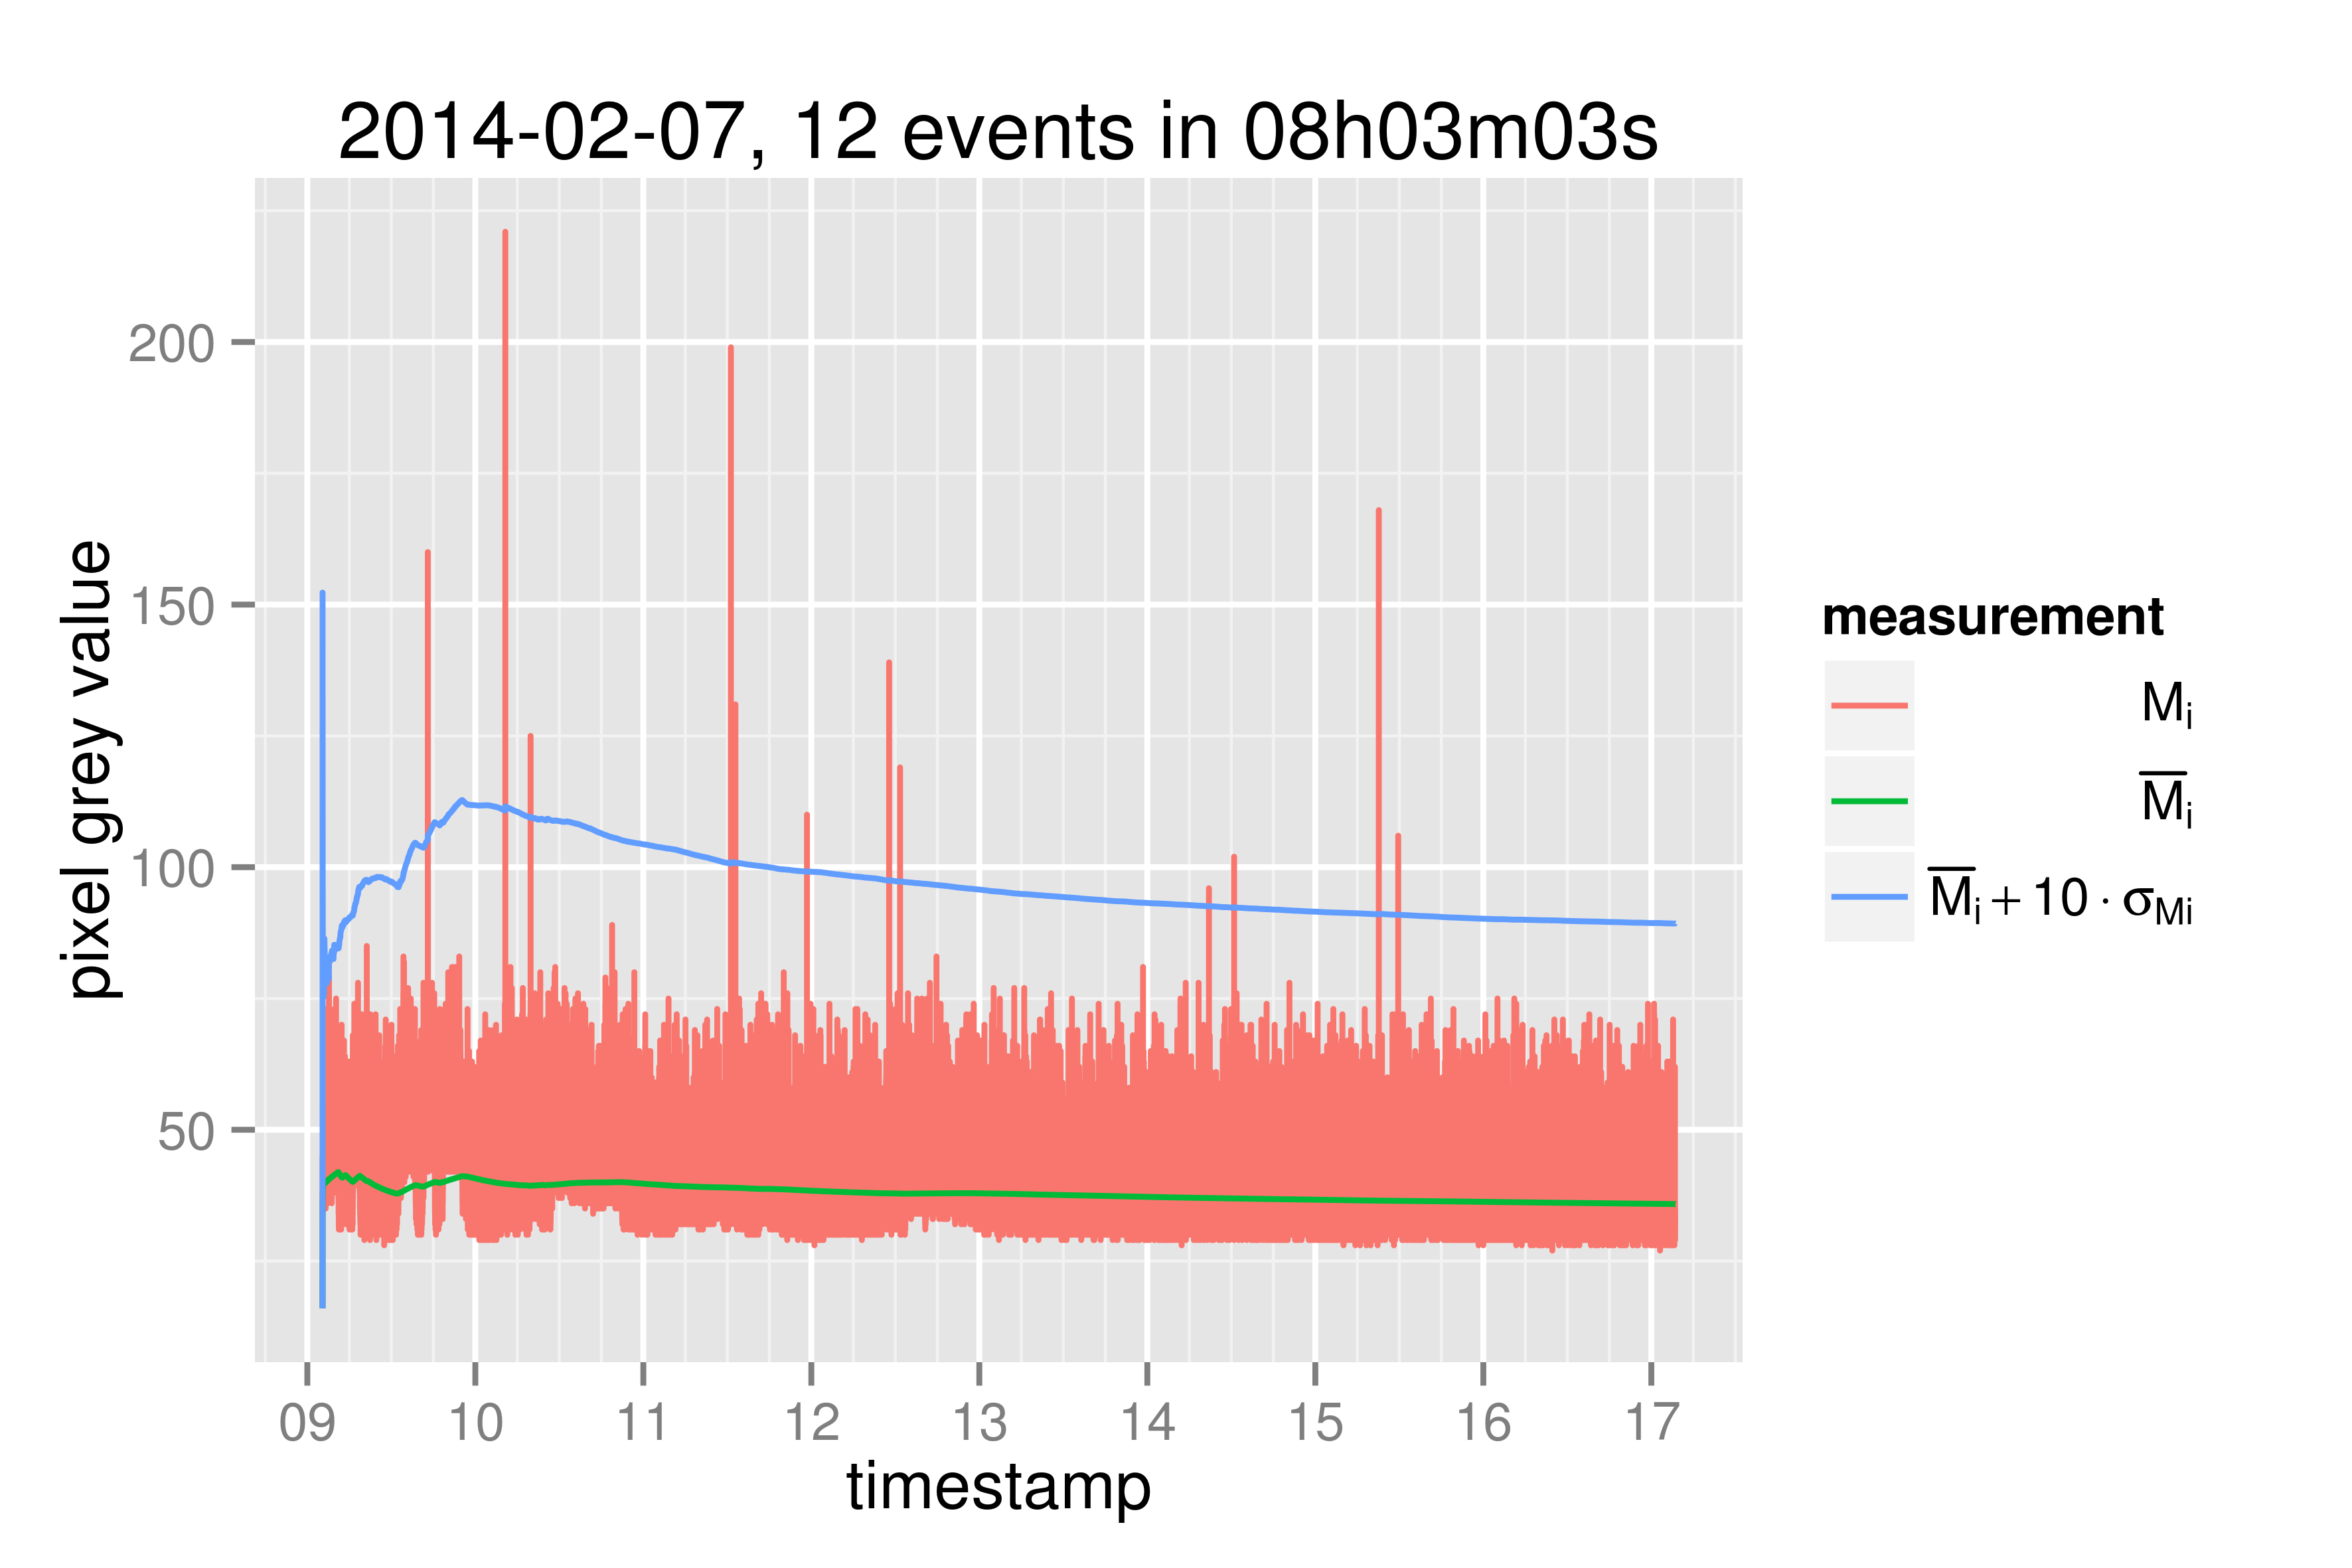
\includegraphics{20140207.png}
  \caption{Data collected using formula \ref{eq:3} with $n=10$.}
\end{figure}

\begin{figure}[h!]
  \centering
  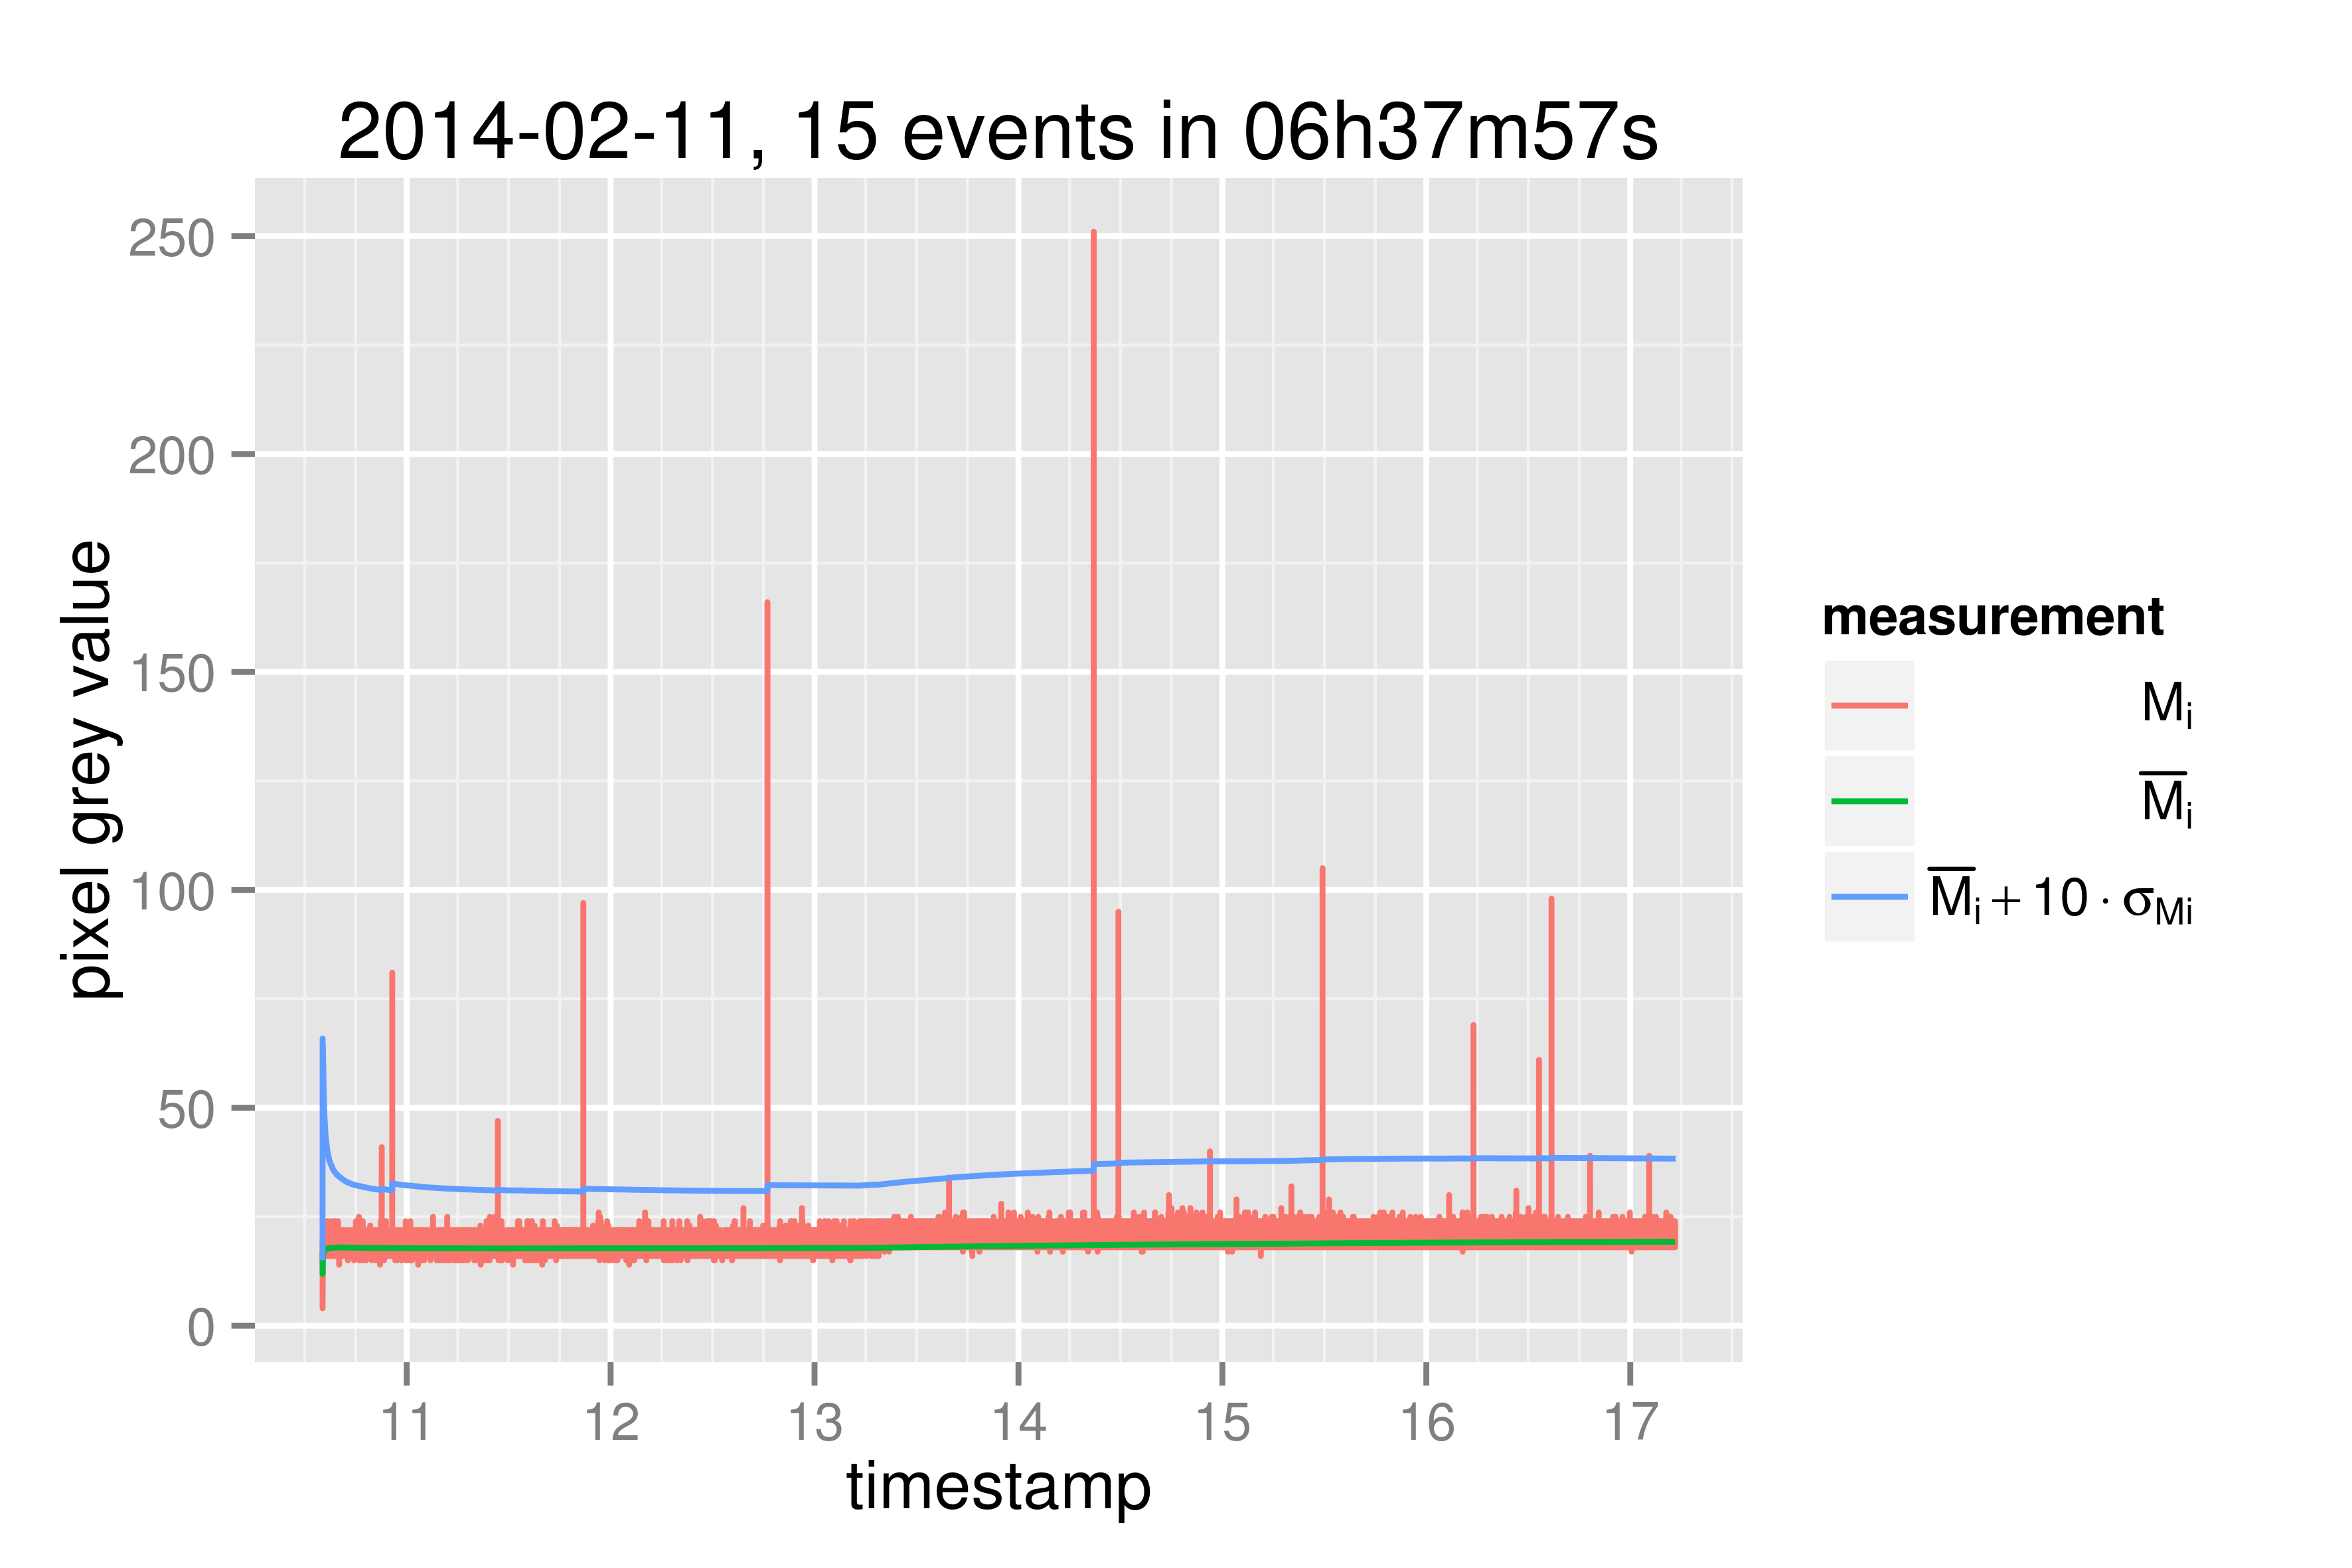
\includegraphics{20140211.png}
  \caption{Data collected using formula \ref{eq:3} with $n=10$.}
\end{figure}

\begin{figure}[h!]
  \centering
  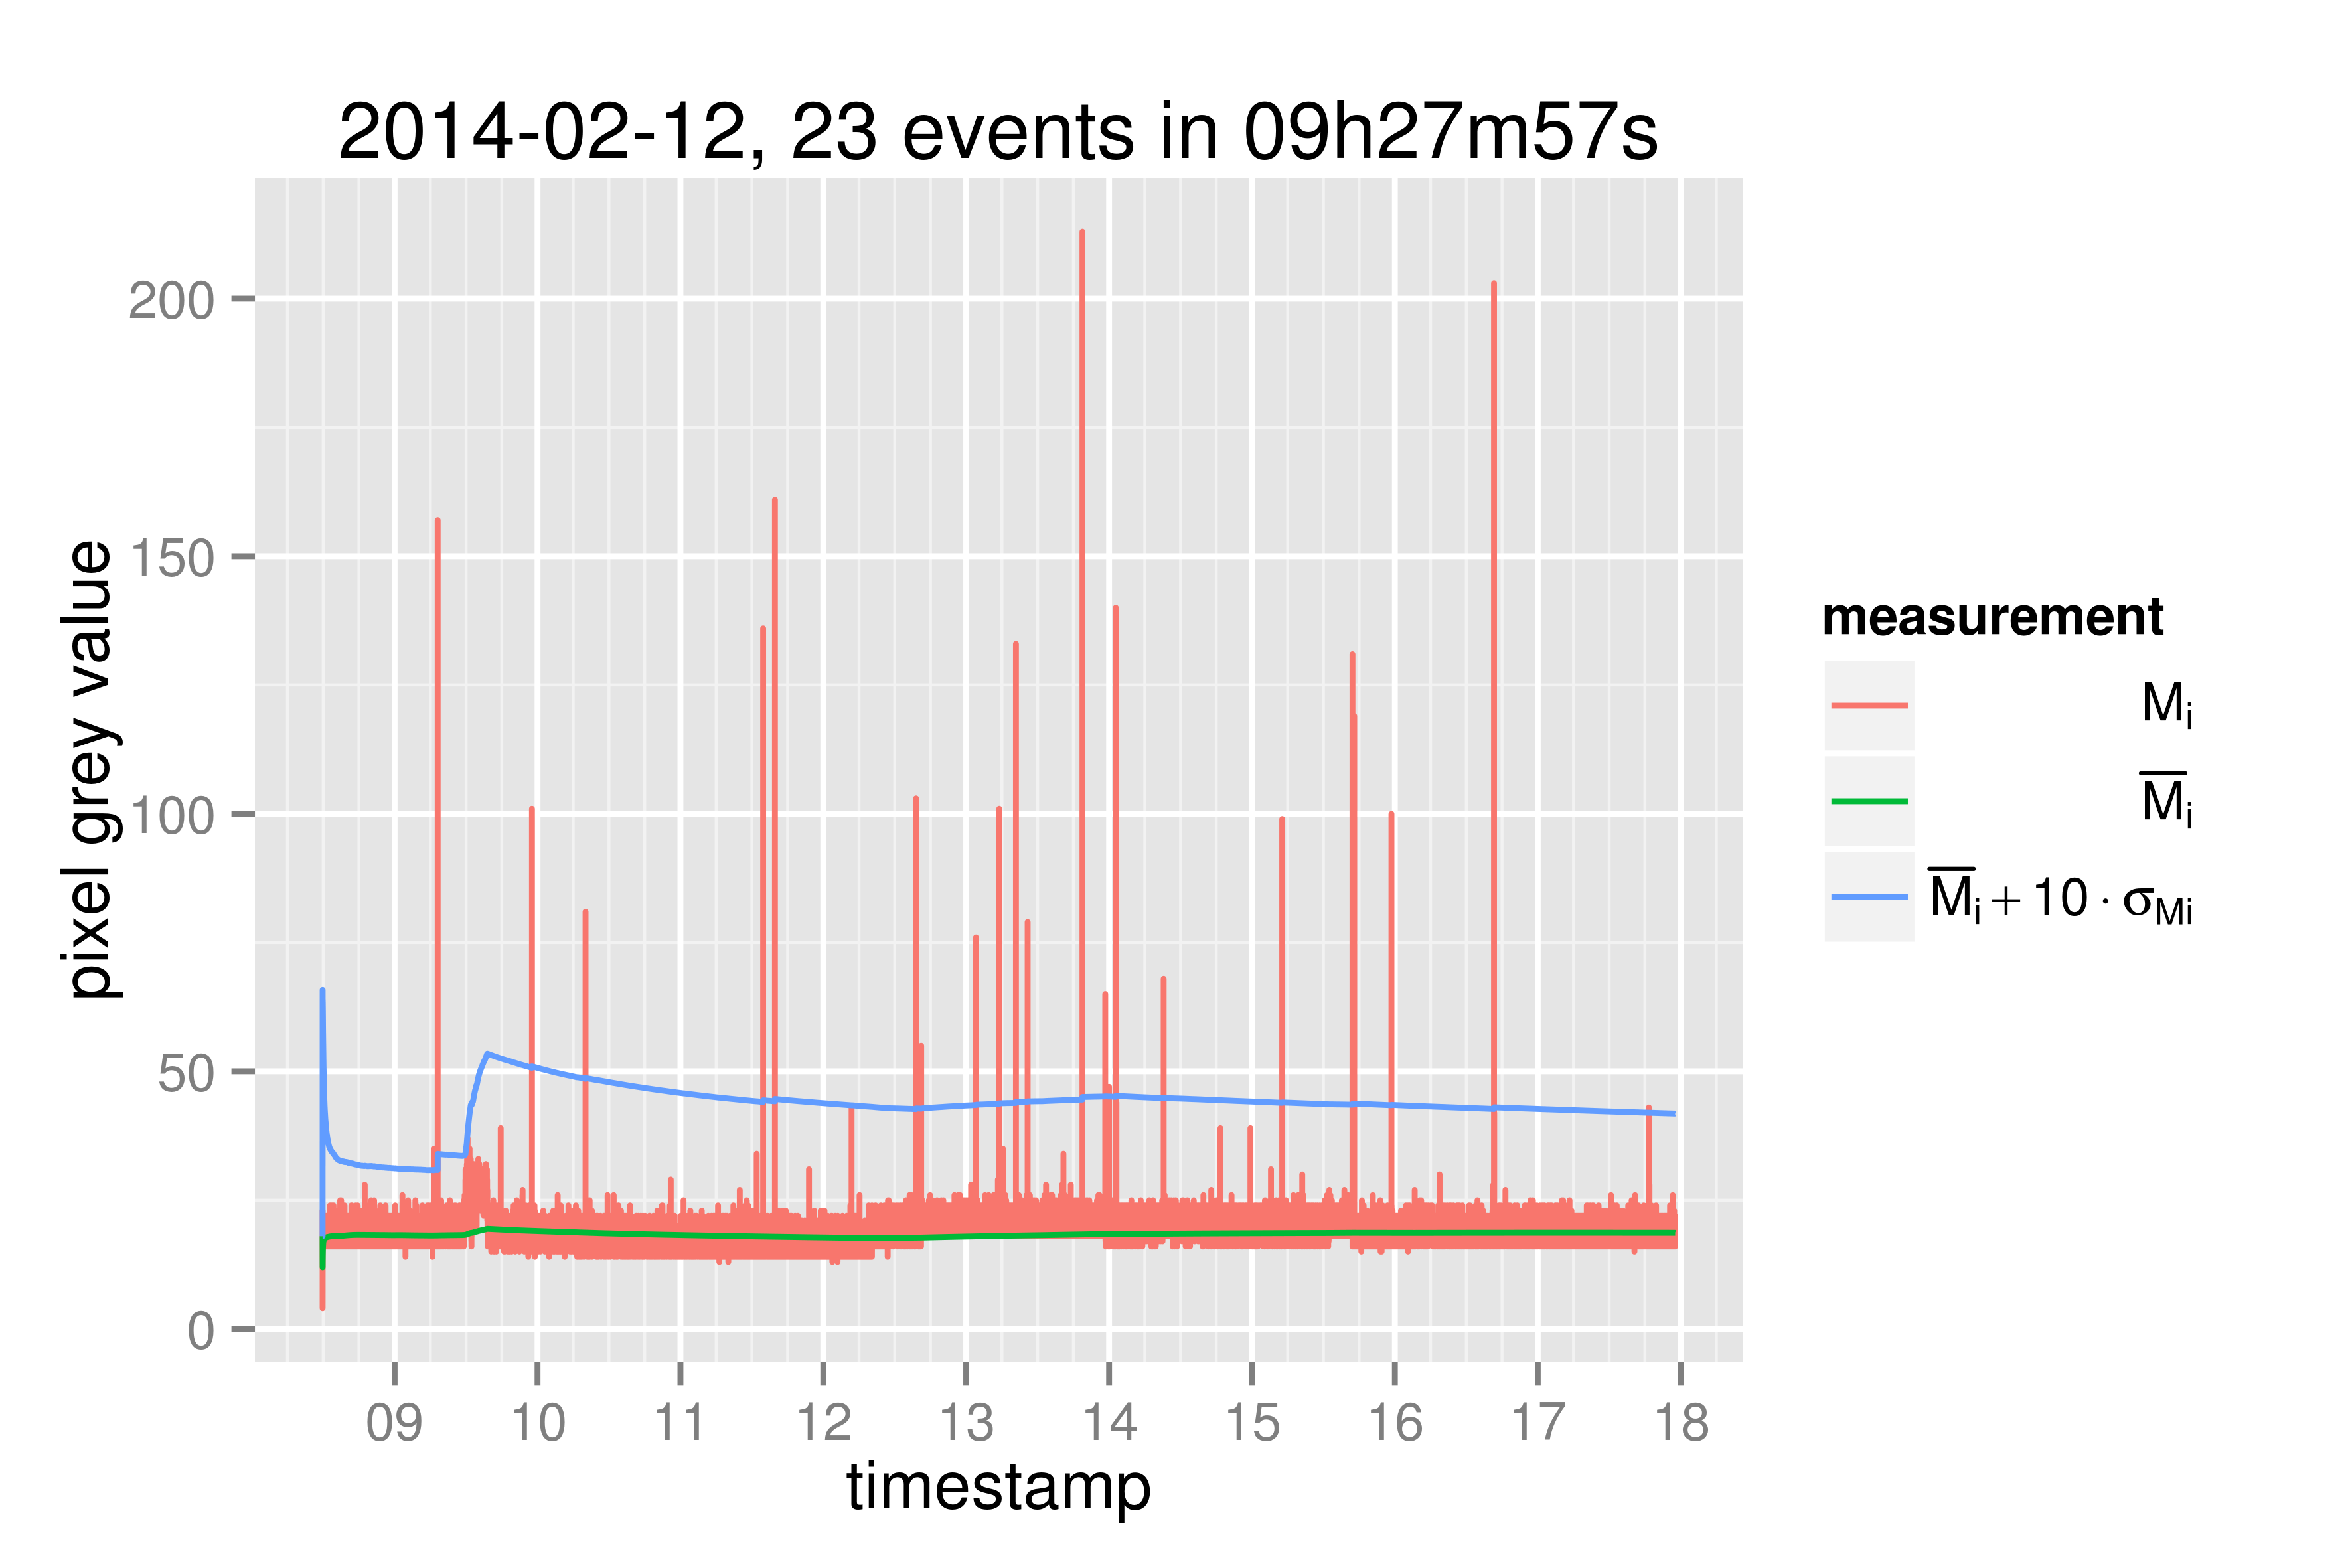
\includegraphics{20140212.png}
  \caption{Data collected using formula \ref{eq:3} with $n=10$.}
\end{figure}

\begin{figure}[h!]
  \centering
  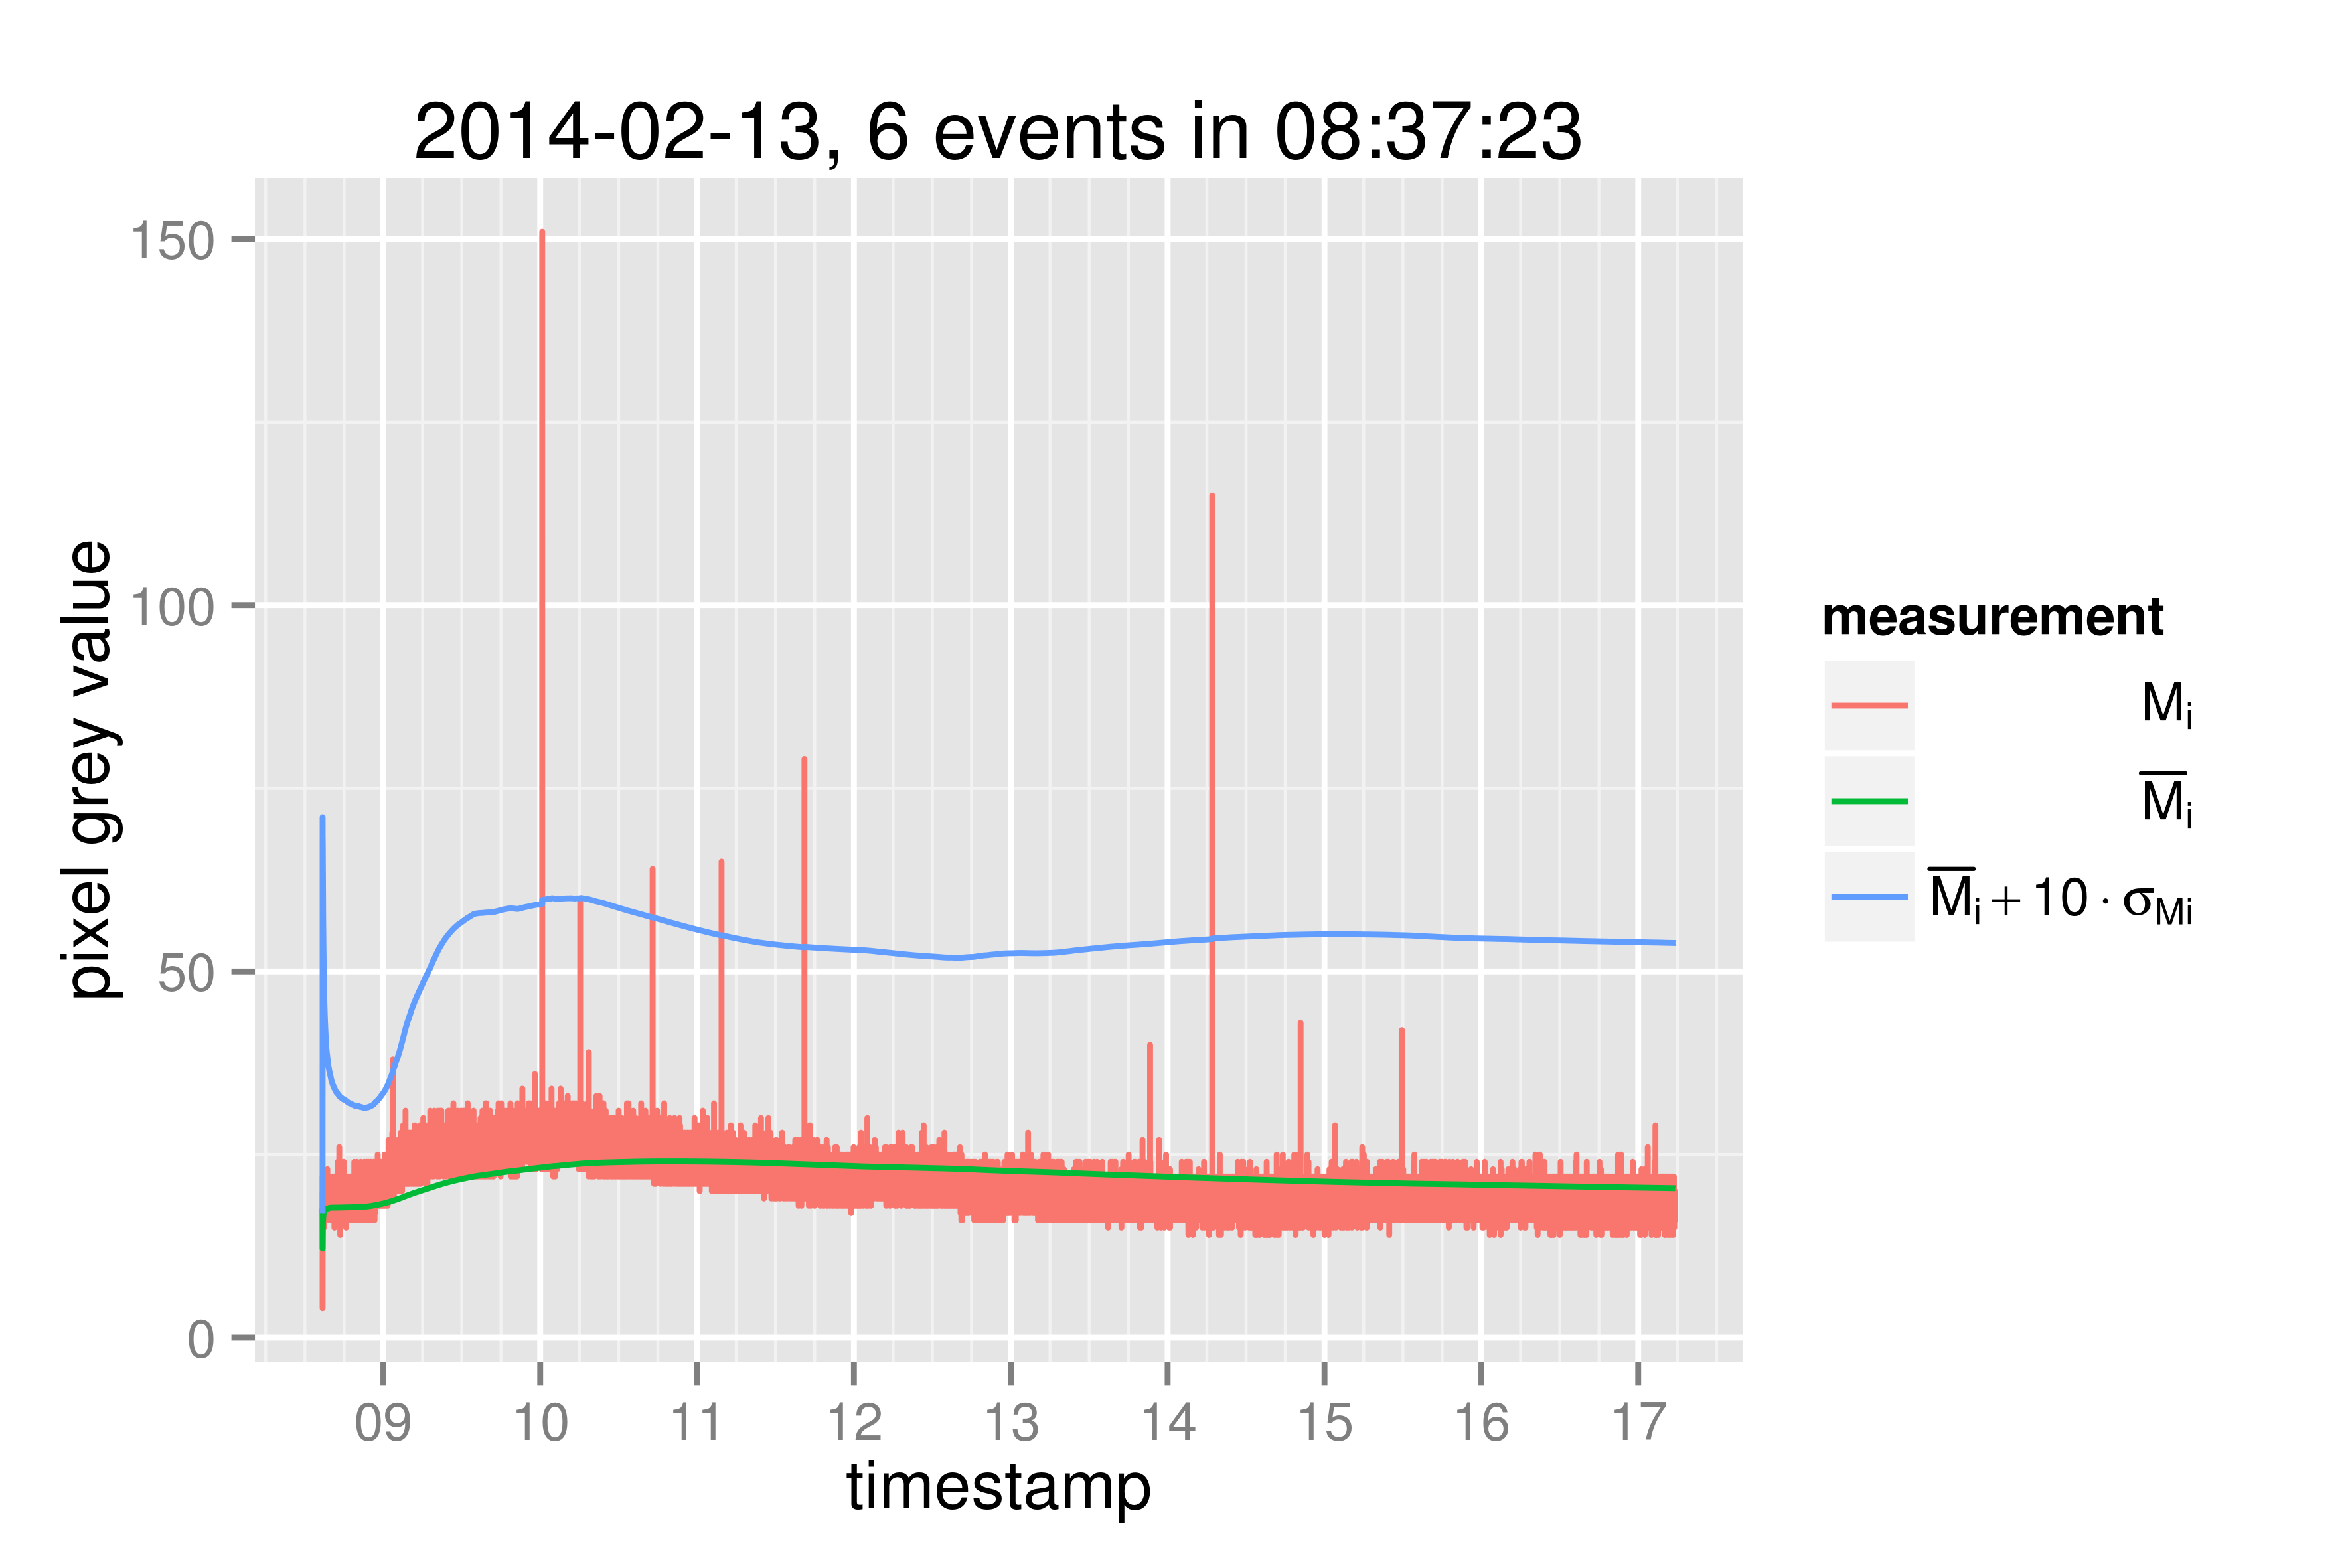
\includegraphics{20140213.png}
  \caption{Data collected using formula \ref{eq:3} with $n=10$.}
\end{figure}

\begin{figure}[h!]
  \centering
  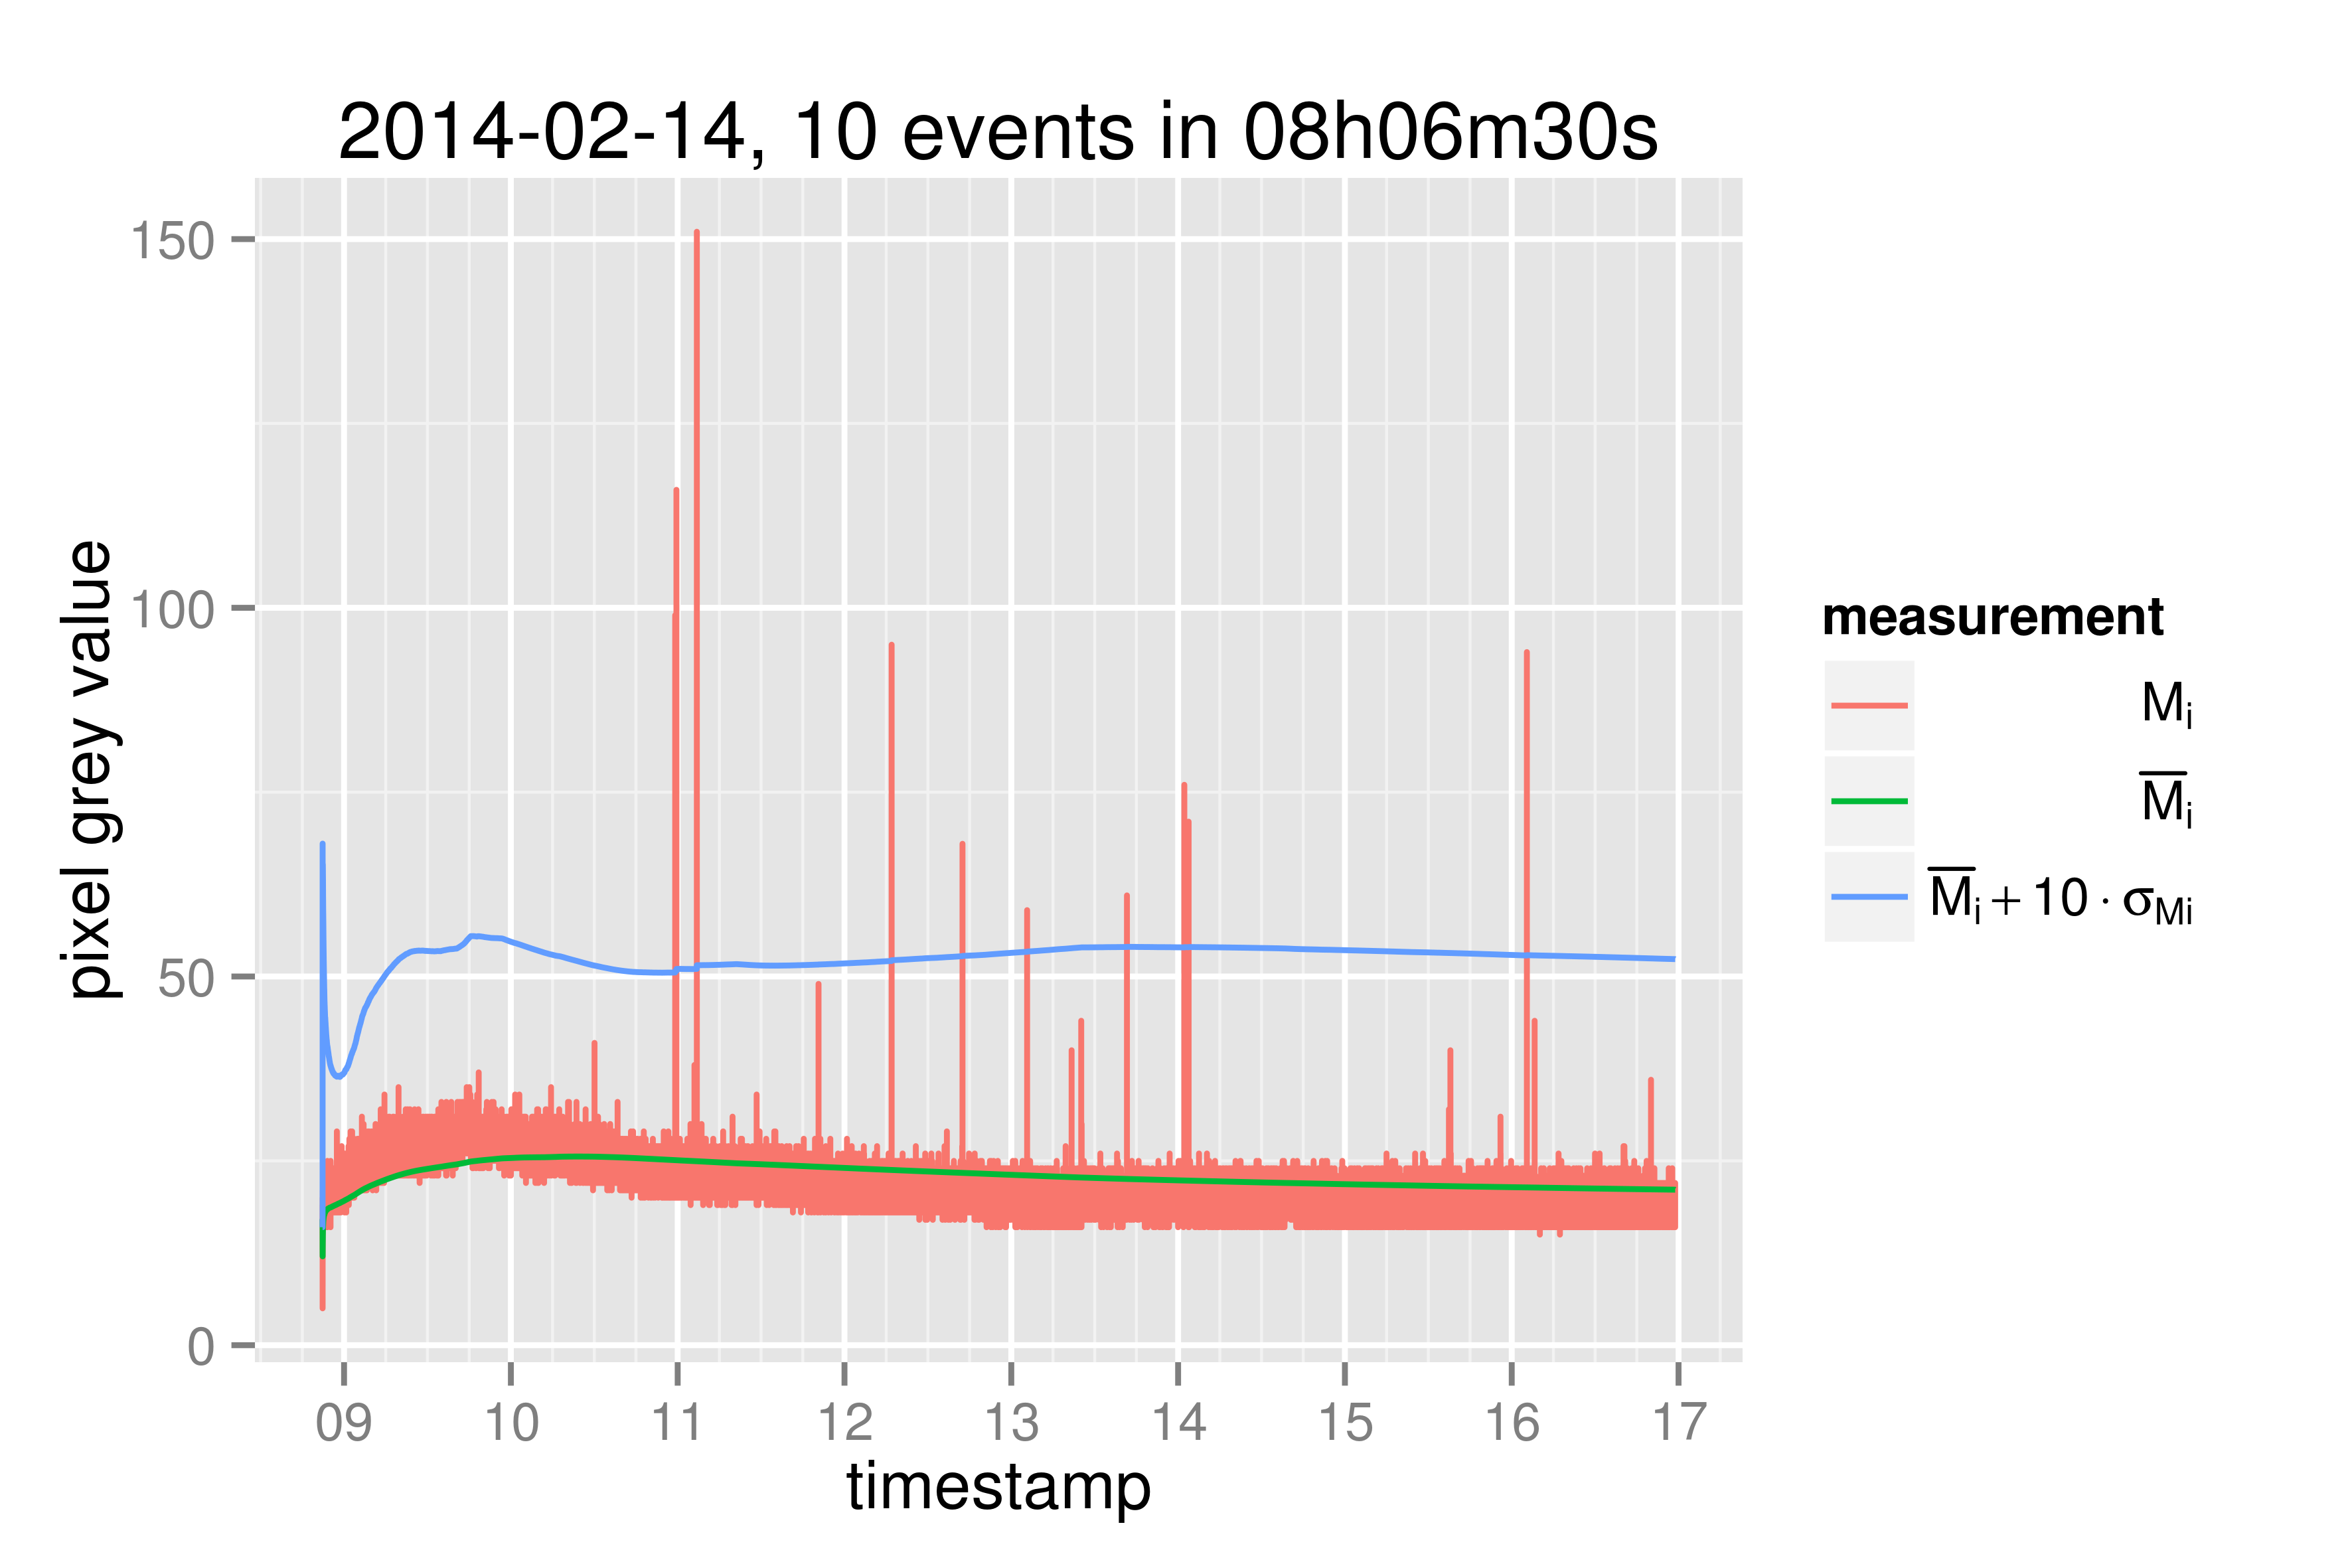
\includegraphics{20140214.png}
  \caption{Data collected using formula \ref{eq:3} with $n=10$.}\label{fig:2}
\end{figure}

\end{document}
